\documentclass[11pt, a4paper]{article}
\usepackage[utf8]{inputenc}
\usepackage{amsmath,setspace,geometry}
\usepackage{amsfonts}
\usepackage[shortlabels]{enumitem}
\usepackage{rotating}
\usepackage{pdflscape}
%\usepackage[dvipdfmx]{hyperref,graphicx}
\usepackage{graphicx}
\usepackage{bbm}
\usepackage[dvipsnames]{xcolor}
\usepackage[colorlinks=true, linkcolor= BrickRed, citecolor = BrickRed, filecolor = BrickRed, urlcolor = BrickRed, hypertexnames = true]{hyperref}
\usepackage[]{natbib} 
\bibpunct[:]{(}{)}{,}{a}{}{,}
\geometry{left = 1.0in,right = 1.0in,top = 1.0in,bottom = 1.0in}
%\onehalfspacing
% \usepackage{setspace}
%\doublespacing
%\renewcommand{\baselinestretch}{0.3}
\usepackage[english]{babel}
\usepackage{float}
\usepackage{subfig}
\usepackage{booktabs}
\usepackage{pdfpages}
\usepackage{threeparttable}
\usepackage{lscape}
\usepackage{bm}
\setstretch{1.4}



\newtheorem{theorem}{Theorem}
\newtheorem{assumption}{Assumption}
\newtheorem{lemma}{Lemma}
\newtheorem{definition}{Definition}
\newtheorem{proposition}{Proposition}
\newtheorem{claim}{Claim}
\newtheorem{corollary}{Corollary}
\newtheorem{example}{Example}

\title{Revisiting Conduct
Parameter Estimation in Homogeneous Goods Markets\textcolor{blue}{: Linear Model is A Valid Specification.}}
\author{Yuri Matsumura\footnote{Department of Economics, Rice University. Matsumura: \texttt{\href{mailto:Yuri.Matsumura@rice.edu}{Yuri.Matsumura@rice.edu}}} \and Suguru Otani \footnote{Department of Economics, Rice University. Otani: \texttt{\href{mailto:so19@rice.edu}{so19@rice.edu}}}}

\begin{document}

\maketitle

\begin{abstract}
    We revisit the conduct parameter estimation in homogeneous goods market. In contrast to the pessimistic simulation results shown in \cite{perloff2012collinearity}, our simulation shows that the estimation becomes accurate by properly adding demand shifters in the supply estimation and increasing the sample size. We also investigate log-linear models widely used in Industrial Organization literature and recommended by \cite{perloff2012collinearity} and find other estimation problems. Based on numerical investigation, we recommend using a linear model as a valid specification . %As a remedy, we propose MPEC approach \citep{su2012constrained,dube2012improving} for simultaneous equation GMM with inequality constraint and show its robustness to the DGP.
\end{abstract}

\section{Introduction}
%主題%
Measuring competitiveness in markets is one of the important tasks in Empirical Industrial Organization (IO) literature.
Conduct parameter is regarded as a useful measure of competitiveness. 
However, it cannot be measured directly from data because data usually lack information about marginal cost.
Therefore, the researchers have tried to identify and estimate the conduct parameter.

The literature has considered two popular specifications of the model for conduct parameter estimation in homogeneous good markets; one is the model with linear demand and linear marginal cost and the other is the model with log-linear demand and log-linear marginal cost.\footnote{As a similar strand of the literature, there is growing literature on conduct parameter estimation in differentiated goods markets. For example, see \cite{gandhi2021empirical}.}

%現状 - 1%
As for the linear model, \citet{bresnahan1982oligopoly} considers the identification of conduct parameter in this model. 
\citet{perloff2012collinearity} show that the model in \citet{bresnahan1982oligopoly} is suffering from the multicollinearity problem when the error terms in the demand and supply equations are zero and claim that the model parameters cannot be estimated.
While the situation where the multicollinearity problem arises hardly happens not only in simulation studies but also in practice, the paper still claims that the nearly perfect collinearity contaminates the estimation.
By conducting Monte Carlo simulations, the paper shows that the marginal cost parameters and the conduct parameter cannot be accurately estimated.
To avoid the multicollinearity problem and nearly perfect collinearity, the paper recommends using log-linear or some other functional form for at least one of the equations.

%現状 - 2%
As for the log-linear model, which is recommended by \cite{perloff2012collinearity} as a valid specification for identification, the identification strategy is provided by \citet{lau1982identifying}. The specification is often used in the empirical papers such as \cite{okazaki2022excess} and \cite{merel2009measuring}.

%問題 -1%
We find that there are several problems and misunderstanding for both the linear and log linear model.
As for the linear model, we find that the simulation in \cite{perloff2012collinearity} has two problems.
First, their estimation of the supply equation lacks an excluded demand shifter.
Second, the paper does not check the effect of increasing the sample size. 
%問題 - 2%
As for the log linear model, to the best of our knowledge, there is no simulation study to justify the claim of \cite{perloff2012collinearity}.
\cite{hyde1995can} conduct a simulation of the model, but the paper does not show the simulation result itself. Instead, the result of hypothesis tests based on the simulation result.
However, the simulation still has the same problem in \cite{perloff2012collinearity} because it lacks the demand shifter in the supply-side estimation.

%結果%
Given these problems in the simulations, we revisit the estimation of the conduct parameter in homogeneous product markets.
%To check the accuracy of the estimation of models with the conduct parameter, we reexamine the simulation model in \cite{perloff2012collinearity}.
%To fill in the gap between popular specifications in applied economists and theoretical and numerical discussions, we provide unified numerical simulation results.
First, we replicate the result in \cite{perloff2012collinearity} by complementing some details which they did not mention on instrument construction. 
We confirm that the accuracy of the estimation holds by including a demand shifter in the supply equation estimation properly. 
Given the standard deviation of the error terms, when the sample size is more than 100, the accuracy of the estimation is also improved.
In this sense, \cite{perloff2012collinearity} provides correct theoretical results but incorrect numerical simulation results.

Second, we conduct the simulation of the model with log-linear demand and log-linear marginal cost that is suggested by \cite{perloff2012collinearity}. 
We numerically show that standard OLS regression estimates an incorrect conduct parameter out of range of $[0,1]$ because the specification may add another identification problem of the conduct parameter and constant term of marginal costs. 
The nonidentification results of the log-linear specification are mistakenly reported in IO literature as imprecise estimation results, for example, \cite{okazaki2022excess}. 
Thus, we conclude that the linear specification is a valid specification for the conduct parameter estimation in homogeneous good markets.


\section{Model}
The researcher has data with $T$ markets with homogeneous products.
Assume that there are $N_t$ firms in each market.
Let $t = 1,\ldots, T$ be the index of markets and $j = 1, \ldots, N_t$ be the index of firms in market $t$.
Firm $j$ solves a profit maximization problem such that
\begin{align}
    \max_{q_{jt}} \ \pi_{jt}(q_{jt}, q_{-jt}) \equiv (P(Q_t) - mc_{jt}(q_{jt}))q_{jt},\nonumber
\end{align}
where $Q_t = \sum_{j = 1}^{N_t} q_{jt}$ is the aggregate quantity, $P(Q_t)$ the inverse demand function, and $mc_{jt}(q_{jt})$ the marginal cost function.
From the maximization problem, we obtain the first-order condition,
\begin{align}
    0 = P(Q_{t}) - mc_{jt}(q_{jt}) + \theta_i P'(Q_{t})q_{jt},\nonumber
\end{align}
where $\theta_{it} = 1 + \sum_{k\ne j}\frac{\partial q_{kt}}{\partial q_{jt}}$, which is called conduct parameter.
\textcolor{blue}{By summing up the first-order condition across firms}, we obtain the supply equation 
\begin{align}
     P_t = -\theta_{t}P'(Q_{t})Q_t + MC_t(Q_t)\label{eq:supply_relation}
\end{align}
where $\theta_t = \frac{1}{N_t}\sum_{i = 1}^{N_t}\theta_{it}$ and $MC_t(Q_t) = \frac{1}{N_t}\sum_{j = 1}^{N_t} mc_{jt}(q_{jt})$.

Let's consider an econometric model of the quantity competition.
Assume that the demand function and the marginal cost function are written as 
\begin{align}
    P_t = f(Q_t, Y_t, \varepsilon_{dt}, \alpha) \label{eq:demand}\\
    MC_t = g(Q_t, W_t, \varepsilon_{ct}, \gamma)\label{eq:marginal_cost}
\end{align}
where $Y_t$ and $W_t$ are the vector of exogenous variables, $\varepsilon_{dt}$ and $\varepsilon_{ct}$ the error terms, and $\alpha$ and $\gamma$ are the vector of parameters
We also have the vector of the demand-side instrument variables $Z_{dt}$ and the vector of the supply-side instrument variables $Z_{ct}$.
Then we assume that the error terms satisfy the mean independence condition $E[\varepsilon_{dt}\mid Y_t, Z_{dt}] = E[\varepsilon_{ct} \mid W_t, Z_{ct}] =0$.


\section{Identification of the conduct parameter}
The identification of the conduct parameter in a linear model is considered by \cite{bresnahan1982oligopoly} and the identification in a general model which includes the log model is considered by \cite{lau1982identifying}.
Here we review the identification in \cite{bresnahan1982oligopoly} to see the importance of an instrument variable called the demand rotation IV.

Assume that the demand function \eqref{eq:demand} and the marginal cost function \eqref{eq:marginal_cost} are linear
\begin{align}
    P_{t}=\alpha_0 - \alpha_1 Q_{t} + \alpha_2 Y_t + \varepsilon_{dt},\\
    MC_{t} = \gamma_0 + \gamma_1 Q_t + \gamma_3 W_t + \varepsilon_{ct}.
\end{align}
As we have the demand-side instruments $Z_{dt}$, we can identify the parameters in the demand equation easily and regard the value of the parameters as given.
Now consider the identification of the parameter in the supply equation.
By substituting $\partial P_t/\partial Q_t = - \alpha_1$ into the supply equation \eqref{eq:supply_relation}, we obtain
\begin{align}
    P_{t}&=\gamma_0+\gamma_1 Q_t + \theta\alpha_1 Q_t + \gamma_3 Y_t + \varepsilon_{ct} =\gamma_0+\left(\gamma_1- \theta\alpha_1\right) Q_t + \gamma_3 Y_t + \varepsilon_{ct} \nonumber
\end{align}
Then, the value of $(\gamma_1- \theta\alpha_1)$ is identified, but $\theta$ and $\gamma_1$ cannot be identified separately.

\cite{bresnahan1982oligopoly} provides the trick to identify $\theta$. 
Assume that the inverse demand is given as 
\begin{align}
    P_{t}=\alpha_0 - (\alpha_1+\alpha_2 Z^R_t) Q_{t} + \alpha_3 Y_t + \varepsilon_{dt},
\end{align}
where $Z^R_t$ is called demand rotation IV.
Again, the demand parameters are identified.
By substituting $\partial P_t/\partial Q_t = -(\alpha_1+\alpha_2 Z^R_t)$ into the supply equation \eqref{eq:supply_relation}, we obtain
\begin{align}
    P_{t}&=\gamma_0+\gamma_1 Q_t + \theta (\alpha_1+\alpha_2 Z^R_t) Q_t + \gamma_3 W_t + \varepsilon_{ct} \nonumber\\
    &= \gamma_0 + (\gamma_1 + \theta \alpha_1) Q_t + \theta\alpha_1 Z^R_tQ_t + \gamma_3 W_t + \varepsilon_{ct}   \nonumber
\end{align}
Since $\alpha_1$ and $\alpha_2$ are identified from the demand equation and $(\gamma_1 + \theta\alpha_1)$ and $\theta \alpha_1$ are identified, we can identify $\theta$ and $\gamma_1$ separately.



\section{Simulation and Estimation Setting}\label{sec:simulation_and_estimation_setting}

\subsection{Linear demand and linear cost}
Assume that a linear demand function and a linear marginal cost function such that
\begin{align}
    P_t &= \alpha_0 - (\alpha_1 + \alpha_2Z^R_t)Q_t + \alpha_3 Y_t + \varepsilon_{dt},\label{eq:linear_demand}\\
    MC_t &= \gamma_0  + \gamma_1 Q + \gamma_2 w_t + \gamma_3 r_t + \varepsilon_{ct},\label{eq:linear_marginal_cost}
\end{align}
where $w_t$ and $r_t$ are excluded cost shifter.
\textcolor{blue}{The supply equation is given as}
\begin{align}
    P_t = \gamma_0 + [\theta(\alpha_1 + \alpha_2Z^R_t)+ \gamma_1] Q_t   + \gamma_2 w_t + \gamma_3 r_t + \varepsilon_{ct}\label{eq:linear_supply_equation}
\end{align}
By substituting the linear demand equation \eqref{eq:linear_demand} into the supply equation \eqref{eq:linear_supply_equation}, we can represent the aggregate quantity $Q_t$ based on the parameters and the exogenous variables as   
\begin{align}
    Q_t =  \frac{\alpha_0 + \alpha_3 Y_t - \gamma_0 - \gamma_2 w_t - \gamma_3 r_t + \varepsilon_{dt} - \varepsilon_{ct}}{(1 + \theta) (\alpha_1 + \alpha_2Z^R_t) + \gamma_1}.
\end{align}

Assume that the exogenous and instrument variables are drawn from normal distributions; $ Y_t \sim N(0,1)$, $w_t \sim N (3, 1)$, $r_t \sim N (0, 1)$, $ Z^R_t \sim N (10, 1)$.
\textcolor{blue}{As additional instruments, two random variables are created by adding an additional random variable drawn from the standard normal distribution to $w_t$ and $r_t$, which is denoted by $h_t$ and $k_t$.}
% The value of the conduct parameter is $\theta = 0.5$, the value of the constant term in the demand equation is $\alpha_0 = 10$, and the value of the rest of the parameters is one; $\alpha_1 = \alpha_2 = \alpha_3 = \gamma_0 = \gamma_1 = \gamma_2  = \gamma_3 = 1$. 
% The error terms follow the normal distribution with mean zero and with standard deviation $\sigma$; $\varepsilon_{ct}\sim N(0,\sigma)$, $\varepsilon_{dt} \sim N(0,\sigma)$.
% We change the value of $\sigma$ to see how the variation of the error terms affects the accuracy of the estimation.







\subsection{Log demand and log marginal cost}

Considers a model with log demand and a Cobb-Douglas cost function. 
The log demand equation and log marginal cost are given as:
\begin{align}
    \log P_{t} &= \alpha_0 - (\alpha_1 + \alpha_2 Z^R_t) \log Q_t + \alpha_3 \log Y_t + \varepsilon_{dt},\label{eq:log_linear_demand}\\
    \log MC_t &= \gamma_0 + \gamma_1 \log Q_t +  \gamma_2 \log w_t + \gamma_3 \log r_t + \varepsilon_{ct}.\label{eq:log_linear_marginal_cost}
\end{align}
Since $\partial P_t/\partial Q_t = - (\alpha_1 + \alpha_2 Z^R) (P_t/Q_t) $, \textcolor{blue}{the supply equation is given as:}
\begin{align}
    P_t &= \theta_t (\alpha_1 + \alpha_2 Z^R_t) \frac{P_t}{Q_t} Q_t + mc_t.\label{eq:log_linear_supply_equation}
\end{align}
\textcolor{blue}{By taking logarithm???}, we obtain
\begin{align}
    \log P_t = - \log(1 - \theta(\alpha_1 + \alpha_2 Z^R_t)) + \gamma_0 + \gamma_1 \log Q_t +  \gamma_2 \log w_t + \gamma_3 \log r_t + \varepsilon_{ct} \label{eq:supply_equation_loglinear}
\end{align}
By substituting the log linear demand equation \eqref{eq:log_linear_demand} into the supply equation \eqref{eq:log_linear_supply_equation}, the log aggregate quantity is given as 
\begin{align}
    \log Q_t &= \frac{ \alpha_0 + \alpha_3 \log Y_t + \log (1 - \theta (\alpha_1 + \alpha_2 Z^R_t)) - \gamma_0  -  \gamma_2 \log w_t - \gamma_3 \log r_t + \varepsilon_{dt} - \varepsilon_{ct}}{\gamma_1+ \alpha_1 + \alpha_2 Z^R_t }.
\end{align}


% Assume that the exogenous in the cost side and instrument variables are drawn from uniform distributions; $w \sim U(1,3)$, $r \sim U(0,1)$, and $Z \sim U(0, 1)$. 
% The demand shifter $Y_t$ is drawn from the standard normal distribution.
% The error terms are drawn from a normal distribution with mean zero and standard deviation $\sigma$; $\varepsilon_{ct}\sim N(0,\sigma)$, $\varepsilon_{dt} \sim N(0,\sigma)$.
% The value of the conduct parameter is $\theta = 0.3$, the value of $\alpha_0$ and $\alpha_2$ in the demand equation are $\alpha_0 = 10, \alpha_2 = 0.1$, and the value of the rest of the parameters is one; $\alpha_1 = \alpha_3 = \gamma_0 = \gamma_1 = \gamma_2  = \gamma_3 = 1$.
% The similar specification is investigated in \cite{hyde1995can}.

\subsection{Parameter and distribution setting}

We set the true parameters and distributions as in Table \ref{tb:parameter_setting}. 
As for the linear specification, we follow the setting of \cite{perloff2012collinearity} \textcolor{blue}{except for the coefficient of the demand shifter XXX.}
As for the log linear specification, we need to use different DGP from the linear specification to generate reasonable data through the logarithmic transformation. 
We confirm that the both settings provide downward log demand curves.
The similar specification is investigated in \cite{hyde1995can}.
We change the value of $\sigma$ to see how the variation of the error terms affects the accuracy of the estimation.


\begin{table}[!htbp]
    \caption{True parameters and distributions}
    \label{tb:parameter_setting}
    
    \begin{center}
    \subfloat[Parameters]{
    \begin{tabular}{crr}
            \hline
            & linear & log linear \\
            $\alpha_0$ & $10.0$ & $10.0$ \\
            $\alpha_1$ & $1.0$ & $1.0$  \\
            $\alpha_2$ & $1.0$ & $0.1$ \\
            $\alpha_3$ & $1.0$ & $1.0$ \\
            $\gamma_1$ & $1.0$ & $1.0$  \\
            $\gamma_2$ & $1.0$ & $1.0$ \\
            $\gamma_3$ & $1.0$ & $1.0$ \\
            $\theta$ & $0.5$ & $0.3$  \\
            \hline
        \end{tabular}
    }
    \subfloat[Distribution]{
    \begin{tabular}{crr}
            \hline
            & linear & log linear \\
            Demand shifter&  &  \\
            $Y_t$ & $N(0,1)$ & $N(0,1)$ \\
            $h_t$ & $N(0,1)$ & $U(0,1)$  \\
            $k_t$ & $N(0,1)$ & $U(0,1)$  \\
            Rotation demand shifter&  &  \\
            $Z_t$ & $N(10,1)$ & $U(0,1)$ \\
            Cost shifter&  &  \\
            $w_t$ & $N(3,1)$ & $U(1,3)$ \\
            $r_t$ & $N(0,1)$ & $U(0,1)$  \\
            Error&  &  \\
            $\varepsilon_{dt}$ & $N(0,\sigma)$ & $N(0,\sigma)$  \\
            $\varepsilon_{ct}$ & $N(0,\sigma)$ & $N(0,\sigma)$ \\
            \hline
        \end{tabular}
    }
    \end{center}
    \footnotesize
    Note: $\sigma=\{0.001, 0.5, 1.0, 2.0\}$. $N:$ Normal distribution. $U:$ Uniform distribution.
\end{table}





% \subsubsection{Estimation in Hyde and Perloff (1995)}
% The demand and supply equations are
% \begin{align}
%     &\log P_{t} = \alpha_0 - \alpha_1 \log Q_t - \alpha_2 Z^R_t\log Q_t + \alpha_3 \log Y_t + \varepsilon_{dt},\\
%     &\log P_t  = - \log(1 - \theta(\alpha_1 + \alpha_2 Z^R_t)) + \gamma_0 + \gamma_1 \log Q_t +  \gamma_2 \log w_t + \gamma_3 \log r_t + \varepsilon_{ct}.
% \end{align}
% As we can immediately see, the supply equation is a nonlinear equation.
% We assume two moment conditions $E[Z_{dt} \varepsilon_{dt}] = \bm0 $ and $ E[Z_{ct} \varepsilon_{ct}] =\bm0$ where $Z_{dt}$ is the vector of instruments for the demand equation and $Z_{ct}$ the vector of instruments for the supply equation.
% Based on the moment conditions, we can apply the generalized method of moments.
% We consider two estimators; the nonlinear system 2SLS estimator and the nonlinear 3SLS estimator.\footnote{See Wooldridge (2010), Ch 14.}


\subsection{Estimation procedure}
%To estimate the parameters in the demand equation and the supply equation, \cite{perloff2012collinearity} applies the 2SLS, the 3SLS, and the nonlinear 3SLS.
%Since \cite{perloff2012collinearity} only shows the results based on the 2SLS and the 3SLS, we also focus on these estimation methods.

The estimation of both the linear model and the log-linear model is based on the 2SLS estimation.
The instrument variables for the demand estimation are $Z_{dt} = (Z^R_t, Y_t, h_t, k_t)$ and the instrument variables for the supply estimation are $Z_{ct} = (Z^R_t, w_t, r_t, Y_t)$.

To conduct the simulation of the linear model, we generate 1000 data sets by using R and estimate the equations by using the \texttt{ivreg} package in R.
We separately estimate the demand and the supply equation.
Note that an important feature of the model is that we have an interaction term of the endogenous variable $Q_t$ and the instrument variable $Z^R_t$.
The \texttt{ivreg} package automatically detects that the endogenous variables are $Q_t$ and the interaction term $Z^R_tQ_t$ and runs the first stage regression for each endogenous variable by using the same instruments.
\footnote{To confirm this, we manually wrote R code that implements the 2SLS. 
When the first stage includes only the regression of $Q_t$, the estimation results from our code differ from the results from \texttt{ivreg}. 
But when we modified the code so that regress $Z^R_tQ_t$ on the instrument variables and estimate the second stage by using the predicted values of $Q_t$ and $Z^R_tQ_t$, the result from our code and the result from \texttt{ivreg} coincided.}

To conduct the simulation of the log-linear model, we also generate 1000 data sets by using R. 
For estimation, we estimate the demand parameters as in the linear model by using R since the demand equation is linear.
In contrast, for estimation of the cost parameters, we use Julia and apply the generalized method of moments (GMM) with the moment condition $E[Z_{ct} \varepsilon_{ct}] = 0$ since the supply side equation is nonlinear.
Note that for the supply estimation, we substitute the demand estimation result.
The GMM estimator is obtained as a solution to the minimization problem.\footnote{For the detail, see Ch.14 of \citet{wooldridge2010econometric}.}
To solve the minimization problem, we formulate the minimization problem via \texttt{JuMP.jl} and solve the problem by using the nonlinear solver \texttt{IPOPT.jl}.



\section{Results}

\subsection{The linear demand and linear marginal cost model}

\begin{table}[!htbp]
    \caption{Estimation results in Table 2 of from \cite{perloff2012collinearity}}
    \label{tb:linear_linear_sigma_Perloff_Shen}
    \begin{center}
        \begin{tabular}{cllll}
            \hline
            & $\sigma=0.001$ & $\sigma=0.5$ & $\sigma=1$ & $\sigma=2$ \\
            $\alpha_0$ & $10.00\ (0.001)$ & $9.96\ (0.33)$ & $9.86\ (0.65)$ & $9.46(1.20)$ \\
            $\alpha_1$ & $1.00\ (0.004)$ & $0.99\ (1.98)$ & $0.97\ (3.96)$ & $0.88(7.80)$ \\
            $\alpha_2$ & $1.00\ (0.004)$ & $0.99\ (0.21)$ & $0.97\ (0.42)$ & $0.87\ (0.82)$ \\
            $\gamma_1$ & $0.46\ (0.88)$ & $0.46\ (0.91)$ & $0.47\ (0.93)$ & $0.49\ (1.04)$ \\
            $\gamma_2$ & $5.85\ (7.89)$ & $5.85\ (8.15)$ & $5.78\ (8.21)$ & $5.73\ (8.66)$ \\
            $\theta$ & $-0.31\ (1.31)$ & $-0.29\ (1.34)$ & $0.09\ (11.48)$ & $-1.53\ (30.41)$ \\
            \hline
        \end{tabular}
    \end{center}\footnotesize
    Note: True parameters: $\alpha_1 = \alpha_2 = \gamma_0 = \gamma_1 = \gamma_2  = \gamma_3 = 1, \alpha_0 = 10, \alpha_3 = 0,  \theta = 0.5$. \citet{perloff2012collinearity} exclude $Y_t$. We change the parameter notations from the original paper.
\end{table}

First, we replicate the result in \citet{perloff2012collinearity}.
The simulation setting in \cite{perloff2012collinearity} is different from our simulation setting; while we assume that the value of the coefficient $\alpha_3$ of $Y_t$ is one, \cite{perloff2012collinearity} does not include $Y_t$ to generate their simulation data and assumes $\alpha_3 = 0$.
In this case, any exogenous demand shifter is used for the supply estimation.

Table \ref{tb:linear_linear_sigma_Perloff_Shen} is quoted from \cite{perloff2012collinearity}, although we modify some notations.
The sample size in each simulation data is 50 and the table shows the mean and the standard deviation of the 2SLS estimators from 1000 simulations.
It shows that the demand estimation becomes accurate as the value of the standard deviation of the error terms $\sigma$ decreases.
In contrast, the supply-side estimation is still biased and the standard deviation of the conduct parameter becomes larger as the value of $\sigma$ increases.

Table \ref{tb:linear_linear_sigma_1_without_demand_shifter_y} shows our replication results.
Each panel shows the simulation result under different standard deviations of the error terms.
This result uses the same data generation process with \citet{perloff2012collinearity}, but for the estimation, we complement what the authors do not mention on instrument construction.
To see if we can correctly replicate the result in \cite{perloff2012collinearity}, let's focus on the first two columns in each panel.
These two columns show the mean and the standard deviation of the simulation result when the sample size is 50.
The result is while the demand parameter can be accurately estimated even though the value of $\sigma$ becomes larger, the supply side parameter is biased.
Especially, when $\sigma$ is large and the sample size is small, the standard deviation of the parameters in the supply-side equation becomes large.
Thus we can correctly replicate the result in \citet{perloff2012collinearity}.
As \cite{perloff2012collinearity} fixes its sample size to 50, we also see the effect of changing the sample size.
As it is expected, the increase in the sample size given a value of $\sigma$ decreases the value of the standard deviation of the parameter in the supply equation.
But no simulation result is close to the true values of the supply parameter and the conduct parameter.
These results are consistent with \cite{perloff2012collinearity}.

However, we show that their pessimistic result can be easily resolved just by adding a demand shifter and increasing the sample size.
Table \ref{tb:linear_linear_sigma_1} shows the 2SLS estimation results with the demand shifter.
The results are based on the simulation setting explained in Section \ref{sec:simulation_and_estimation_setting}.
When $\sigma = 0.001$, Panel (a) shows that the estimation of all parameters is quite accurate.
Especially, when the sample size is large, the standard deviations of all parameters are less than 0.001.
When $\sigma = 2$ and the sample size is 50, Panel (d) shows that the supply-side estimation is still biased.
The value of $\gamma_1$, the coefficient of $Q_t$ in the supply equation, is far from the true value $\gamma_1 = 1$ and the standard deviation is much larger than the standard deviation in the model without $Y_t$.
But as the sample size increases, the standard deviation is dramatically improved, and when the sample size is 1000, all parameters are estimated more accurately than the result in the model without $Y_t$.

\begin{table}[!htbp]
  \begin{center}
      \caption{Estimation results of the linear model without demand shifter}
      \label{tb:linear_linear_sigma_1_without_demand_shifter_y} 
      \subfloat[$\sigma=0.001$]{
\begin{tabular}[t]{lrrrrrrrr}
\toprule
  & (1) $n=50$ / Mean & (1) $n=50$ / SD & (2) $n=100$ / Mean & (2) $n=100$ / SD & (3) $n=200$ / Mean & (3) $n=200$ / SD & (4) $n=1000$ / Mean & (4) $n=1000$ / SD\\
\midrule
$\alpha_{0}$ & 10.000 & 0.0009 & 10.000 & 0.0006 & 10.000 & 0.0004 & 10.000 & 0.0002\\
$\alpha_{1}$ & 1.000 & 0.004 & 1.000 & 0.003 & 1.000 & 0.002 & 1.000 & 0.0009\\
$\alpha_{2}$ & 1.000 & 0.0005 & 1.000 & 0.0003 & 1.000 & 0.0002 & 1.000 & 0.0001\\
$\gamma_{0}$ & 5.446 & 6.981 & 5.388 & 7.986 & 5.423 & 7.825 & 5.063 & 6.801\\
$\gamma_{1}$ & 0.506 & 0.775 & 0.512 & 0.888 & 0.509 & 0.869 & 0.549 & 0.756\\
$\gamma_{2}$ & 0.506 & 0.776 & 0.512 & 0.887 & 0.509 & 0.869 & 0.549 & 0.756\\
$\theta$ & -0.241 & 1.164 & -0.231 & 1.331 & -0.237 & 1.304 & -0.177 & 1.134\\
$R^{2}$ (demand) & 1.000 & 0.0000004 & 1.000 & 0.0000003 & 1.000 & 0.0000002 & 1.000 & 8e-08\\
$R^{2}$ (supply) & 1.000 & 0.000008 & 1.000 & 0.00001 & 1.000 & 0.00001 & 1.000 & 0.000008\\
Sample size ($T$) &  & 50 &  & 100 &  & 200 &  & 1000\\
\bottomrule
\end{tabular}
}\\
      \subfloat[$\sigma=0.5$]{
\begin{tabular}[t]{lrrrrrrrr}
\toprule
  & (1) $n=50$ / Mean & (1) $n=50$ / SD & (2) $n=100$ / Mean & (2) $n=100$ / SD & (3) $n=200$ / Mean & (3) $n=200$ / SD & (4) $n=1000$ / Mean & (4) $n=1000$ / SD\\
\midrule
$\alpha_{0}$ & 9.993 & 0.466 & 9.993 & 0.312 & 10.001 & 0.215 & 10.002 & 0.093\\
$\alpha_{1}$ & 0.963 & 2.138 & 0.965 & 1.484 & 1.012 & 1.023 & 0.991 & 0.441\\
$\alpha_{2}$ & 1.002 & 0.243 & 1.002 & 0.168 & 0.999 & 0.118 & 1.002 & 0.049\\
$\gamma_{0}$ & 5.332 & 10.459 & 5.227 & 11.592 & 5.112 & 15.871 & 5.470 & 7.476\\
$\gamma_{1}$ & 0.405 & 3.214 & 0.434 & 1.989 & 0.474 & 1.744 & 0.516 & 1.102\\
$\gamma_{2}$ & 0.517 & 1.157 & 0.528 & 1.222 & 0.546 & 1.816 & 0.504 & 0.830\\
$\theta$ & -0.210 & 1.879 & -0.206 & 1.951 & -0.186 & 2.705 & -0.247 & 1.238\\
$R^{2}$ (demand) & 0.720 & 0.088 & 0.725 & 0.061 & 0.726 & 0.041 & 0.728 & 0.018\\
$R^{2}$ (supply) & 0.160 & 7.674 & -0.119 & 19.529 & -0.724 & 30.775 & 0.491 & 2.041\\
Sample size (n) &  & 50 &  & 100 &  & 200 &  & 1000\\
\bottomrule
\end{tabular}
}\\
  \end{center}\footnotesize
  Note: True parameters: $\alpha_1 = \alpha_2 =  \gamma_0 = \gamma_1 = \gamma_2  =  1, \alpha_0 = 10, \theta = 0.5.$ and $\alpha_3 =0$
\end{table} 

\begin{table}[!htbp]
  \ContinuedFloat  %% <-- new
  \begin{center}
      \caption{Estimation results of the linear model without demand shifter (Continued)}
      \label{tb:linear_linear_sigma_1_without_demand_shifter_y} 
      \subfloat[$\sigma=1.0$]{
\begin{tabular}[t]{lrrrrrrrr}
\toprule
  & Mean & SD & Mean  & SD  & Mean   & SD   & Mean    & SD   \\
\midrule
$\alpha_{0}$ & 9.975 & 0.964 & 9.953 & 0.636 & 10.007 & 0.441 & 9.991 & 0.189\\
$\alpha_{1}$ & 1.120 & 4.491 & 0.942 & 2.885 & 0.883 & 2.055 & 1.035 & 0.902\\
$\alpha_{2}$ & 0.981 & 0.492 & 0.993 & 0.326 & 1.015 & 0.227 & 0.993 & 0.101\\
$\gamma_{0}$ & 5.631 & 9.410 & 5.520 & 7.580 & 5.161 & 9.226 & 5.556 & 7.424\\
$\gamma_{1}$ & -0.107 & 19.285 & 0.129 & 5.240 & 0.488 & 3.541 & 0.489 & 1.210\\
$\gamma_{2}$ & 0.476 & 1.043 & 0.495 & 0.835 & 0.540 & 1.030 & 0.494 & 0.820\\
$\theta$ & -0.201 & 3.603 & -0.217 & 1.478 & -0.183 & 1.528 & -0.260 & 1.229\\
$R^{2}$ (demand) & 0.205 & 0.357 & 0.234 & 0.221 & 0.232 & 0.150 & 0.245 & 0.060\\
$R^{2}$ (supply) & -0.920 & 17.898 & -0.395 & 5.271 & -0.904 & 12.486 & -0.421 & 12.047\\
Sample size (n) &  & 50 &  & 100 &  & 200 &  & 1000\\
\bottomrule
\end{tabular}
}\\
    \subfloat[$\sigma=2.0$]{
\begin{tabular}[t]{lrrrrrrrr}
\toprule
  & Mean & SD & Mean  & SD  & Mean   & SD   & Mean    & SD   \\
\midrule
$\alpha_{0}$ & 9.515 & 6.752 & 9.912 & 1.479 & 9.987 & 0.943 & 9.987 & 0.396\\
$\alpha_{1}$ & 0.362 & 19.344 & 0.710 & 6.192 & 1.154 & 4.363 & 0.986 & 1.728\\
$\alpha_{2}$ & 0.934 & 1.092 & 1.004 & 0.743 & 0.981 & 0.494 & 0.998 & 0.204\\
$\gamma_{0}$ & 5.658 & 6.892 & 5.464 & 8.387 & 5.695 & 8.243 & 5.572 & 10.796\\
$\gamma_{1}$ & 0.956 & 52.166 & 1.715 & 42.062 & -0.056 & 11.467 & 0.388 & 3.140\\
$\gamma_{2}$ & 0.479 & 0.827 & 0.496 & 0.907 & 0.486 & 0.902 & 0.497 & 1.185\\
$\theta$ & -0.296 & 5.941 & -0.439 & 5.106 & -0.235 & 2.034 & -0.256 & 1.771\\
$R^{2}$ (demand) & -3.456 & 87.362 & -0.513 & 1.557 & -0.436 & 0.563 & -0.376 & 0.185\\
$R^{2}$ (supply) & -1.104 & 5.881 & -2.311 & 26.606 & -1.993 & 26.973 & -3.591 & 49.060\\
Sample size ($T$) &  & 50 &  & 100 &  & 200 &  & 1000\\
\bottomrule
\end{tabular}
}
  \end{center}\footnotesize
  Note: True parameters: $\alpha_1 = \alpha_2 =  \gamma_0 = \gamma_1 = \gamma_2  =  1, \alpha_0 = 10, \theta = 0.5.$ and $\alpha_3 =0$
\end{table} 

\begin{table}[!htbp]
  \begin{center}
      \caption{Estimation results of the linear model with demand shifter}
      \label{tb:linear_linear_sigma_1} 
      \subfloat[$\sigma=0.001$]{
\begin{tabular}[t]{lrrrrrrrr}
\toprule
  & (1) $n=50$ / Mean & (1) $n=50$ / SD & (2) $n=100$ / Mean & (2) $n=100$ / SD & (3) $n=200$ / Mean & (3) $n=200$ / SD & (4) $n=1000$ / Mean & (4) $n=1000$ / SD\\
\midrule
$\alpha_{0}$ & 10.000 & 0.0009 & 10.000 & 0.0007 & 10.000 & 0.0004 & 10.000 & 0.0002\\
$\alpha_{1}$ & 1.000 & 0.004 & 1.000 & 0.003 & 1.000 & 0.002 & 1.000 & 0.0009\\
$\alpha_{2}$ & 1.000 & 0.0005 & 1.000 & 0.0003 & 1.000 & 0.0002 & 1.000 & 0.0001\\
$\alpha_{3}$ & 1.000 & 0.0002 & 1.000 & 0.0001 & 1.000 & 0.0001 & 1.000 & 0.00004\\
$\gamma_{0}$ & 1.000 & 0.001 & 1.000 & 0.001 & 1.000 & 0.0007 & 1.000 & 0.0003\\
$\gamma_{1}$ & 1.000 & 0.005 & 1.000 & 0.004 & 1.000 & 0.002 & 1.000 & 0.001\\
$\gamma_{2}$ & 1.000 & 0.0002 & 1.000 & 0.0001 & 1.000 & 0.0001 & 1.000 & 0.00004\\
$\gamma_{3}$ & 1.000 & 0.0002 & 1.000 & 0.0002 & 1.000 & 0.0001 & 1.000 & 0.00005\\
$\theta$ & 0.500 & 0.0006 & 0.500 & 0.0004 & 0.500 & 0.0003 & 0.500 & 0.0001\\
$R^{2}$ (demand) & 1.000 & 0.0000003 & 1.000 & 0.0000002 & 1.000 & 0.0000002 & 1.000 & 7e-08\\
$R^{2}$ (supply) & 1.000 & 0.0000003 & 1.000 & 0.0000002 & 1.000 & 0.0000002 & 1.000 & 7e-08\\
Sample size ($T$) &  & 50 &  & 100 &  & 200 &  & 1000\\
\bottomrule
\end{tabular}
}\\
      \subfloat[$\sigma=0.5$]{
\begin{tabular}[t]{lrrrrrrrr}
\toprule
  & Mean & SD & Mean  & SD  & Mean   & SD   & Mean    & SD   \\
\midrule
$\alpha_{0}$ & 9.982 & 0.465 & 10.007 & 0.323 & 9.992 & 0.213 & 9.994 & 0.097\\
$\alpha_{1}$ & 0.955 & 2.257 & 1.024 & 1.523 & 1.018 & 1.016 & 0.969 & 0.454\\
$\alpha_{2}$ & 0.999 & 0.255 & 0.999 & 0.176 & 0.996 & 0.115 & 1.001 & 0.051\\
$\alpha_{3}$ & 0.995 & 0.108 & 1.003 & 0.075 & 0.999 & 0.050 & 0.999 & 0.022\\
$\gamma_{0}$ & 0.939 & 0.730 & 0.995 & 0.474 & 0.979 & 0.345 & 0.995 & 0.152\\
$\gamma_{1}$ & 0.689 & 3.438 & 0.876 & 1.925 & 0.919 & 1.302 & 0.997 & 0.548\\
$\gamma_{2}$ & 1.009 & 0.109 & 0.999 & 0.071 & 1.003 & 0.051 & 1.000 & 0.023\\
$\gamma_{3}$ & 1.001 & 0.108 & 1.003 & 0.075 & 1.003 & 0.052 & 1.000 & 0.022\\
$\theta$ & 0.547 & 0.351 & 0.517 & 0.208 & 0.514 & 0.134 & 0.503 & 0.058\\
$R^{2}$ (demand) & 0.762 & 0.083 & 0.763 & 0.057 & 0.765 & 0.036 & 0.764 & 0.016\\
$R^{2}$ (supply) & 0.768 & 0.075 & 0.768 & 0.050 & 0.766 & 0.035 & 0.763 & 0.016\\
Sample size (n) &  & 50 &  & 100 &  & 200 &  & 1000\\
\bottomrule
\end{tabular}
}\\
  \end{center}\footnotesize
  Note: True parameters: $\alpha_1 = \alpha_2 = \alpha_3 = \gamma_0 = \gamma_1 = \gamma_2  = \gamma_3 = 1, \alpha_0 = 10, \theta = 0.5.$
\end{table} 

\begin{table}[!htbp]
  \ContinuedFloat  %% <-- new
  \begin{center}
      \caption{Estimation results of the linear model with demand shifter (Continued)}
      \label{tb:linear_linear_sigma_1} 
      \subfloat[$\sigma=1.0$]{
\begin{tabular}[t]{lrrrrrrrr}
\toprule
  & (1) $n=50$ / Mean & (1) $n=50$ / SD & (2) $n=100$ / Mean & (2) $n=100$ / SD & (3) $n=200$ / Mean & (3) $n=200$ / SD & (4) $n=1000$ / Mean & (4) $n=1000$ / SD\\
\midrule
$\alpha_{0}$ & 9.973 & 1.023 & 9.998 & 0.641 & 9.996 & 0.448 & 9.984 & 0.187\\
$\alpha_{1}$ & 0.976 & 4.398 & 0.831 & 2.962 & 1.061 & 2.060 & 1.011 & 0.905\\
$\alpha_{2}$ & 0.994 & 0.495 & 1.016 & 0.324 & 0.993 & 0.234 & 0.994 & 0.100\\
$\alpha_{3}$ & 0.994 & 0.223 & 1.002 & 0.153 & 0.999 & 0.099 & 0.997 & 0.045\\
$\gamma_{0}$ & 0.682 & 1.741 & 0.909 & 1.055 & 0.914 & 0.709 & 0.996 & 0.308\\
$\gamma_{1}$ & 6.859 & 210.877 & 0.321 & 6.247 & 0.662 & 2.954 & 0.950 & 1.109\\
$\gamma_{2}$ & 1.035 & 0.244 & 1.011 & 0.157 & 1.011 & 0.103 & 1.000 & 0.045\\
$\gamma_{3}$ & 1.045 & 0.246 & 1.012 & 0.150 & 1.010 & 0.104 & 1.002 & 0.045\\
$\theta$ & 0.101 & 18.455 & 0.598 & 0.732 & 0.554 & 0.303 & 0.509 & 0.113\\
$R^{2}$ (demand) & 0.301 & 0.409 & 0.305 & 0.199 & 0.310 & 0.134 & 0.319 & 0.054\\
$R^{2}$ (supply) & 0.267 & 0.369 & 0.308 & 0.186 & 0.306 & 0.128 & 0.315 & 0.052\\
Sample size ($T$) &  & 50 &  & 100 &  & 200 &  & 1000\\
\bottomrule
\end{tabular}
}\\
    \subfloat[$\sigma=2.0$]{
\begin{tabular}[t]{lrrrrrrrr}
\toprule
  & (1) $n=50$ / Mean & (1) $n=50$ / SD & (2) $n=100$ / Mean & (2) $n=100$ / SD & (3) $n=200$ / Mean & (3) $n=200$ / SD & (4) $n=1000$ / Mean & (4) $n=1000$ / SD\\
\midrule
$\alpha_{0}$ & 9.737 & 2.584 & 10.071 & 1.669 & 9.960 & 0.947 & 9.998 & 0.412\\
$\alpha_{1}$ & 0.729 & 10.822 & 1.008 & 6.495 & 1.236 & 4.259 & 1.021 & 1.810\\
$\alpha_{2}$ & 0.956 & 1.253 & 1.023 & 0.779 & 0.969 & 0.482 & 0.997 & 0.210\\
$\alpha_{3}$ & 0.976 & 0.584 & 1.008 & 0.343 & 0.996 & 0.225 & 1.003 & 0.092\\
$\gamma_{0}$ & -1.074 & 19.523 & 0.449 & 2.994 & 0.829 & 1.507 & 0.949 & 0.631\\
$\gamma_{1}$ & 59.209 & 1750.596 & -1.416 & 56.886 & -2.617 & 38.895 & 0.897 & 2.333\\
$\gamma_{2}$ & 1.242 & 2.420 & 1.065 & 0.404 & 1.020 & 0.219 & 1.006 & 0.093\\
$\gamma_{3}$ & 1.230 & 2.318 & 1.055 & 0.400 & 1.010 & 0.219 & 1.008 & 0.092\\
$\theta$ & -6.168 & 233.873 & 0.872 & 6.326 & 0.918 & 3.799 & 0.524 & 0.244\\
$R^{2}$ (demand) & -0.653 & 3.934 & -0.513 & 1.300 & -0.363 & 0.518 & -0.319 & 0.191\\
$R^{2}$ (supply) & -10.545 & 132.912 & -0.670 & 1.930 & -0.401 & 0.505 & -0.326 & 0.174\\
Sample size (n) &  & 50 &  & 100 &  & 200 &  & 1000\\
\bottomrule
\end{tabular}
}
  \end{center}\footnotesize
  Note: True parameters: $\alpha_1 = \alpha_2 = \alpha_3 = \gamma_0 = \gamma_1 = \gamma_2  = \gamma_3 = 1, \alpha_0 = 10, \theta = 0.5.$
\end{table} 


\subsection{Log demand and log marginal cost}
Table \ref{tb:loglinear_loglinear_sigma_0.001_separate_non_constraint} provides the simulation results of log-linear demand specifications with a demand shifter. 
We can see that the estimation of the conduct parameter \eqref{eq:supply_equation_loglinear} fails as $\sigma$ becomes large. 
When the standard deviation $\sigma = 0.001$, the estimation results are accurate as in the linear model.
However, when $\sigma$ becomes larger, the mean and the standard deviation of the conduct parameter estimator take unrealistic values.
As the sample size increase, the standard deviation becomes small, but still quite large.




\begin{landscape}
    \begin{table}[!htbp]
      \begin{center}
          \caption{Estimation results of the log linear model with demand shifter}
          \label{tb:loglinear_loglinear_sigma_0.001_separate_non_constraint} 
          \subfloat[$\sigma=0.001$]{
\begin{tabular}[t]{lrrrrrrrr}
\toprule
  & Mean & SD & Mean  & SD  & Mean   & SD   & Mean    & SD   \\
\midrule
$\alpha_{0}$ & 10.000 & 0.004 & 9.998 & 0.004 & 10.001 & 0.002 & 10.000 & 0.001\\
$\alpha_{1}$ & 1.000 & 0.001 & 0.999 & 0.001 & 1.000 & 0.000 & 1.000 & 0.000\\
$\alpha_{2}$ & 0.100 & 0.000 & 0.100 & 0.000 & 0.100 & 0.000 & 0.100 & 0.000\\
$\alpha_{3}$ & 1.000 & 0.000 & 1.000 & 0.000 & 1.000 & 0.000 & 1.000 & 0.000\\
$\gamma_{0}$ & 1.001 & 0.007 & 1.003 & 0.004 & 0.999 & 0.003 & 1.000 & 0.001\\
$\gamma_{1}$ & 1.000 & 0.001 & 1.000 & 0.001 & 1.000 & 0.000 & 1.000 & 0.000\\
$\gamma_{2}$ & 1.000 & 0.001 & 1.000 & 0.000 & 1.000 & 0.000 & 1.000 & 0.000\\
$\gamma_{3}$ & 1.000 & 0.001 & 1.000 & 0.000 & 1.000 & 0.000 & 1.000 & 0.000\\
$\theta$ & 0.098 & 0.004 & 0.099 & 0.002 & 0.100 & 0.002 & 0.100 & 0.001\\
Runs converged (\%) &  & 100.000 &  & 100.000 &  & 100.000 &  & 100.000\\
Sample size ($T$) &  & 50 &  & 100 &  & 200 &  & 1000\\
\bottomrule
\end{tabular}
}\\
          \subfloat[$\sigma=0.5$]{
\begin{tabular}[t]{lrrrrrrrr}
\toprule
  & Mean & SD & Mean  & SD  & Mean   & SD   & Mean    & SD   \\
\midrule
$\alpha_{0}$ & 0.853 & 0.335 & 0.941 & 0.096 & 1.045 & 0.087 & 1.018 & 0.037\\
$\alpha_{1}$ & 0.793 & 0.689 & 0.603 & 0.499 & 0.855 & 0.282 & 0.968 & 0.087\\
$\alpha_{2}$ & 0.557 & 1.532 & 0.415 & 0.418 & 0.241 & 0.350 & 0.136 & 0.207\\
$\alpha_{3}$ & 1.233 & 0.507 & 1.025 & 0.277 & 0.883 & 0.158 & 0.976 & 0.056\\
$\gamma_{0}$ & 1.482 & 0.425 & 1.221 & 0.604 & 1.303 & 0.947 & 1.327 & 0.400\\
$\gamma_{1}$ & 0.888 & 0.381 & 1.198 & 0.349 & 1.027 & 0.276 & 0.929 & 0.081\\
$\gamma_{2}$ & 0.828 & 0.254 & 1.123 & 0.271 & 1.012 & 0.215 & 0.977 & 0.061\\
$\gamma_{3}$ & 0.957 & 0.189 & 1.100 & 0.170 & 1.008 & 0.163 & 0.964 & 0.042\\
$\theta$ & -0.041 & 0.392 & -0.124 & 0.895 & -0.258 & 1.208 & -0.013 & 0.416\\
Runs converged (\%) &  & 80.000 &  & 90.000 &  & 80.000 &  & 90.000\\
Sample size ($T$) &  & 50 &  & 100 &  & 200 &  & 1000\\
\bottomrule
\end{tabular}
}\\
      \end{center}\footnotesize
      Note: True parameters: $\alpha_1 = \alpha_3 = \gamma_0 = \gamma_1 = \gamma_2  = \gamma_3 = 1, \alpha_0 = 10, \alpha_2 = 0.1,  \theta = 0.3.$ 
    \end{table} 
\end{landscape}

\begin{landscape}
    \begin{table}[!htbp]
        \ContinuedFloat  %% <-- new
            \begin{center}
                \caption{Estimation results of the log linear model with demand shifter (Continued)}
                \label{tb:loglinear_loglinear_sigma_0.001_separate_non_constraint} 
                \subfloat[$\sigma=1.0$]{
\begin{tabular}[t]{lrrrrrrrr}
\toprule
  & Mean & SD & Mean  & SD  & Mean   & SD   & Mean    & SD   \\
\midrule
$\alpha_{0}$ & 8.440 & 10.044 & 9.382 & 5.257 & 9.683 & 2.917 & 10.053 & 1.181\\
$\alpha_{1}$ & 0.650 & 2.246 & 0.860 & 1.150 & 0.929 & 0.649 & 1.011 & 0.262\\
$\alpha_{2}$ & 0.081 & 0.255 & 0.096 & 0.136 & 0.096 & 0.073 & 0.101 & 0.031\\
$\alpha_{3}$ & 0.833 & 1.150 & 0.933 & 0.595 & 0.962 & 0.331 & 1.006 & 0.137\\
$\gamma_{0}$ & 4.346 & 6.332 & 4.323 & 5.741 & 3.784 & 5.255 & 2.076 & 3.097\\
$\gamma_{1}$ & 1.015 & 0.371 & 1.020 & 0.233 & 1.021 & 0.158 & 1.004 & 0.067\\
$\gamma_{2}$ & 1.017 & 0.561 & 1.009 & 0.348 & 1.011 & 0.258 & 0.997 & 0.107\\
$\gamma_{3}$ & 1.009 & 0.242 & 1.008 & 0.167 & 1.011 & 0.116 & 1.000 & 0.046\\
$\theta$ & -61173.932 & 1764262.960 & -53104.865 & 252743.866 & -19997.903 & 94198.781 & -2126.896 & 8694.991\\
Solved (%) &  & 0.363 &  & 0.364 &  & 0.466 &  & 0.645\\
Sample size (n) &  & 50 &  & 100 &  & 200 &  & 1000\\
\bottomrule
\end{tabular}
}\\
                \subfloat[$\sigma=2.0$]{
\begin{tabular}[t]{lrrrrrrrr}
\toprule
  & Mean & SD & Mean  & SD  & Mean   & SD   & Mean    & SD   \\
\midrule
$\alpha_{0}$ & 6.416 & 10.448 & 7.385 & 8.342 & 8.366 & 6.582 & 9.953 & 2.371\\
$\alpha_{1}$ & 0.206 & 2.362 & 0.419 & 1.840 & 0.637 & 1.484 & 0.991 & 0.529\\
$\alpha_{2}$ & 0.054 & 0.458 & 0.073 & 0.285 & 0.077 & 0.161 & 0.097 & 0.060\\
$\alpha_{3}$ & 0.613 & 1.169 & 0.699 & 1.287 & 0.824 & 0.713 & 0.996 & 0.270\\
$\gamma_{0}$ & 3.496 & 10.722 & 3.919 & 8.277 & 3.947 & 6.162 & 3.213 & 4.890\\
$\gamma_{1}$ & 1.153 & 1.890 & 1.140 & 1.282 & 1.038 & 0.384 & 1.008 & 0.153\\
$\gamma_{2}$ & 1.098 & 1.669 & 1.003 & 0.762 & 1.007 & 0.526 & 0.998 & 0.233\\
$\gamma_{3}$ & 1.070 & 0.933 & 1.065 & 0.938 & 1.008 & 0.271 & 1.002 & 0.114\\
$\theta$ & -492931.516 & 3240081.766 & -323566.285 & 3240305.105 & -126662.656 & 605408.511 & -15515.297 & 50597.540\\
Solved (%) &  & 0.326 &  & 0.354 &  & 0.389 &  & 0.498\\
Sample size (n) &  & 50 &  & 100 &  & 200 &  & 1000\\
\bottomrule
\end{tabular}
}
            \end{center}\footnotesize
        Note: True parameters: $\alpha_1 = \alpha_3 = \gamma_0 = \gamma_1 = \gamma_2  = \gamma_3 = 1, \alpha_0 = 10, \alpha_2 = 0.1,  \theta = 0.3.$ 
    \end{table} 
\end{landscape}




%\begin{table}[!htbp]
%  \begin{center}
%      \caption{Estimation results with demand shifter with $[0,1]$ constraint on $\theta$ (log-linear)}
%      \label{tb:loglinear_loglinear_sigma_0.001_separate_non_constraint_theta_constraint} 
%      \subfloat[$\sigma=0.001$]{
\begin{tabular}[t]{lrrrrrrrr}
\toprule
  & Mean & SD & Mean  & SD  & Mean   & SD   & Mean    & SD   \\
\midrule
$\alpha_{0}$ & 10.000 & 0.004 & 9.998 & 0.004 & 10.001 & 0.002 & 10.000 & 0.001\\
$\alpha_{1}$ & 1.000 & 0.001 & 0.999 & 0.001 & 1.000 & 0.000 & 1.000 & 0.000\\
$\alpha_{2}$ & 0.100 & 0.000 & 0.100 & 0.000 & 0.100 & 0.000 & 0.100 & 0.000\\
$\alpha_{3}$ & 1.000 & 0.000 & 1.000 & 0.000 & 1.000 & 0.000 & 1.000 & 0.000\\
$\gamma_{0}$ & 1.000 & 0.006 & 1.003 & 0.004 & 0.999 & 0.002 & 0.999 & 0.001\\
$\gamma_{1}$ & 1.000 & 0.001 & 1.000 & 0.001 & 1.000 & 0.000 & 1.000 & 0.000\\
$\gamma_{2}$ & 1.000 & 0.001 & 1.000 & 0.000 & 1.000 & 0.000 & 1.000 & 0.000\\
$\gamma_{3}$ & 1.000 & 0.001 & 1.000 & 0.000 & 1.000 & 0.000 & 1.000 & 0.000\\
$\theta$ & 0.199 & 0.003 & 0.199 & 0.002 & 0.200 & 0.001 & 0.200 & 0.001\\
Runs converged (\%) &  & 100.000 &  & 100.000 &  & 100.000 &  & 100.000\\
Sample size ($T$) &  & 50 &  & 100 &  & 200 &  & 1000\\
\bottomrule
\end{tabular}
}\\
%      \subfloat[$\sigma=0.5$]{
\begin{tabular}[t]{lrrrrrrrr}
\toprule
  & Mean & SD & Mean  & SD  & Mean   & SD   & Mean    & SD   \\
\midrule
$\alpha_{0}$ & 9.271 & 2.598 & 9.777 & 1.664 & 9.989 & 1.289 & 10.017 & 0.508\\
$\alpha_{1}$ & 0.837 & 0.574 & 0.950 & 0.369 & 0.997 & 0.286 & 1.004 & 0.113\\
$\alpha_{2}$ & 0.092 & 0.079 & 0.099 & 0.047 & 0.099 & 0.034 & 0.100 & 0.014\\
$\alpha_{3}$ & 0.919 & 0.294 & 0.972 & 0.189 & 0.999 & 0.149 & 1.001 & 0.059\\
$\gamma_{0}$ & 1.052 & 0.922 & 0.938 & 0.732 & 0.933 & 0.632 & 1.022 & 0.359\\
$\gamma_{1}$ & 0.986 & 0.153 & 0.993 & 0.106 & 0.994 & 0.074 & 0.996 & 0.032\\
$\gamma_{2}$ & 0.980 & 0.247 & 0.990 & 0.177 & 0.995 & 0.121 & 0.997 & 0.054\\
$\gamma_{3}$ & 0.992 & 0.114 & 0.994 & 0.075 & 0.998 & 0.052 & 0.997 & 0.022\\
$\theta$ & 0.289 & 0.354 & 0.335 & 0.342 & 0.308 & 0.289 & 0.267 & 0.201\\
Runs converged (\%) &  & 0.578 &  & 0.607 &  & 0.624 &  & 0.605\\
Sample size ($T$) &  & 50 &  & 100 &  & 200 &  & 1000\\
\bottomrule
\end{tabular}
}\\
%  \end{center}\footnotesize
%  Note: True parameters: $\alpha_1 = \alpha_3 = \gamma_0 = \gamma_1 = \gamma_2  = \gamma_3 = 1, \alpha_0 = 10, \alpha_2 = 0.1,  \theta = 0.3.$
%\end{table} 

%\begin{table}[!htbp]
%  \ContinuedFloat  %% <-- new
%  \begin{center}
%      \caption{Estimation results with demand shifter with $[0,1]$ constraint on $\theta$ (log-linear) (Continued)}
%      \label{tb:loglinear_loglinear_sigma_0.001_separate_non_constraint_theta_constraint} 
%      \subfloat[$\sigma=1.0$]{
\begin{tabular}[t]{lrrrrrrrr}
\toprule
  & Mean & SD & Mean  & SD  & Mean   & SD   & Mean    & SD   \\
\midrule
$\alpha_{0}$ & 7.573 & 4.604 & 8.427 & 4.330 & 9.554 & 2.735 & 10.006 & 1.177\\
$\alpha_{1}$ & 0.339 & 1.217 & 0.579 & 1.158 & 0.883 & 0.734 & 1.000 & 0.313\\
$\alpha_{2}$ & 0.066 & 0.173 & 0.079 & 0.115 & 0.087 & 0.076 & 0.100 & 0.032\\
$\alpha_{3}$ & 0.621 & 0.881 & 0.781 & 0.690 & 0.941 & 0.450 & 0.994 & 0.186\\
$\gamma_{0}$ & 1.319 & 9.549 & 0.134 & 8.964 & 0.315 & 5.079 & 0.655 & 1.264\\
$\gamma_{1}$ & 0.924 & 2.128 & 1.153 & 1.965 & 1.096 & 1.080 & 1.039 & 0.228\\
$\gamma_{2}$ & 0.924 & 1.045 & 1.051 & 0.798 & 1.030 & 0.493 & 1.019 & 0.150\\
$\gamma_{3}$ & 0.922 & 1.144 & 1.054 & 0.880 & 1.039 & 0.528 & 1.010 & 0.150\\
$\theta$ & 0.270 & 0.406 & 0.311 & 0.405 & 0.333 & 0.399 & 0.278 & 0.298\\
Runs converged (\%) &  & 98.500 &  & 98.100 &  & 97.600 &  & 99.900\\
Sample size ($T$) &  & 50 &  & 100 &  & 200 &  & 1000\\
\bottomrule
\end{tabular}
}\\
%    \subfloat[$\sigma=2.0$]{
\begin{tabular}[t]{lrrrrrrrr}
\toprule
  & Mean & SD & Mean  & SD  & Mean   & SD   & Mean    & SD   \\
\midrule
$\alpha_{0}$ & 6.243 & 5.286 & 6.807 & 6.319 & 7.629 & 5.499 & 9.564 & 2.985\\
$\alpha_{1}$ & 0.010 & 1.384 & 0.154 & 1.581 & 0.369 & 1.460 & 0.881 & 0.809\\
$\alpha_{2}$ & 0.040 & 0.313 & 0.056 & 0.252 & 0.060 & 0.179 & 0.094 & 0.068\\
$\alpha_{3}$ & 0.517 & 1.280 & 0.629 & 0.970 & 0.671 & 0.967 & 0.927 & 0.499\\
$\gamma_{0}$ & 4.762 & 17.885 & 2.241 & 17.997 & 1.356 & 9.444 & 0.422 & 2.586\\
$\gamma_{1}$ & 0.209 & 3.820 & 0.741 & 4.079 & 0.903 & 1.972 & 1.069 & 0.503\\
$\gamma_{2}$ & 0.659 & 3.322 & 0.876 & 1.992 & 0.935 & 1.190 & 1.043 & 0.334\\
$\gamma_{3}$ & 0.494 & 5.364 & 0.856 & 2.259 & 0.999 & 1.407 & 1.041 & 0.352\\
$\theta$ & 0.258 & 0.415 & 0.257 & 0.409 & 0.279 & 0.410 & 0.331 & 0.381\\
Runs converged (\%) &  & 98.900 &  & 97.300 &  & 95.900 &  & 97.500\\
Sample size ($T$) &  & 50 &  & 100 &  & 200 &  & 1000\\
\bottomrule
\end{tabular}
}
%  \end{center}\footnotesize
%  Note: True parameters: $\alpha_1 = \alpha_3 = \gamma_0 = \gamma_1 = \gamma_2  = \gamma_3 = 1, \alpha_0 = 10, \alpha_2 = 0.1,  \theta = 0.3.$
%\end{table} 

\section{A problem in log-linear demand specification}



\begin{figure}[!htbp]
  \begin{center}
  \subfloat[]{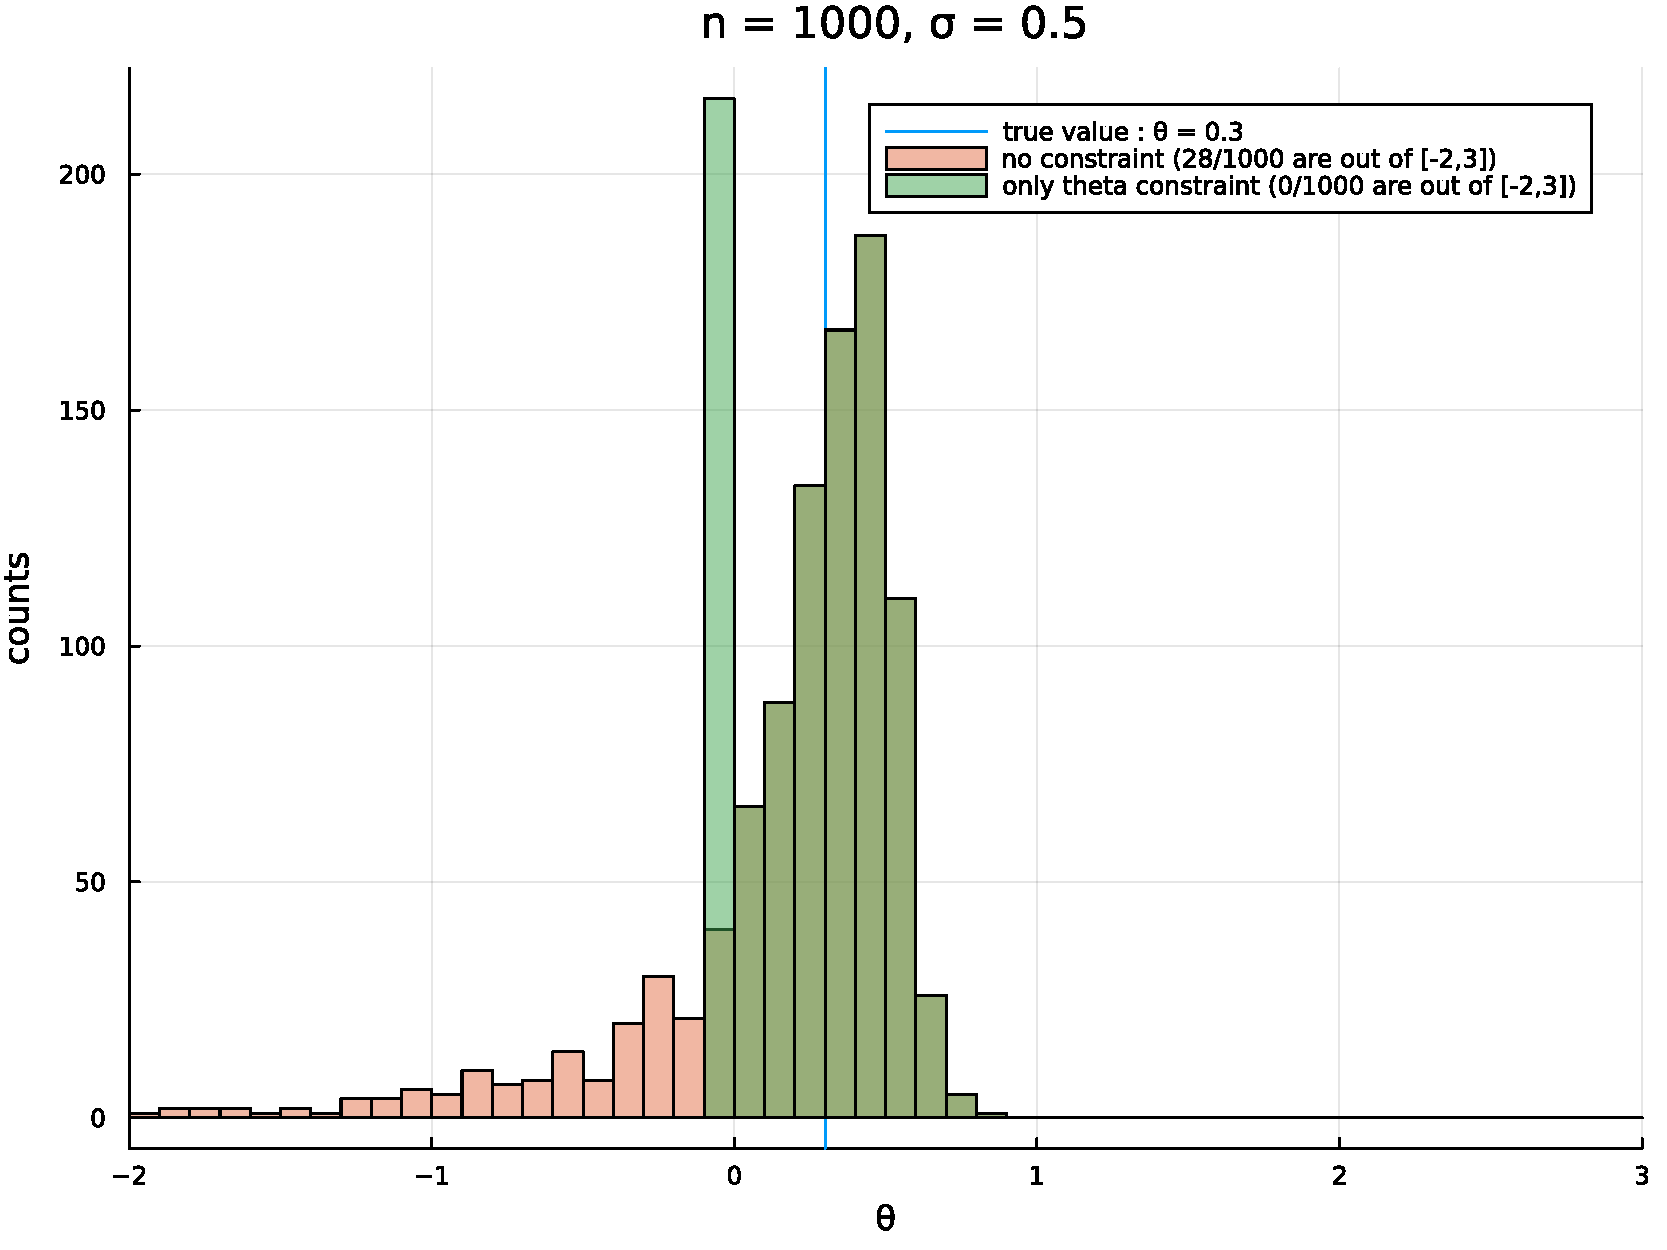
\includegraphics[width = 0.7\textwidth]
  {figuretable/histogram_loglinear_loglinear_n_1000_sigma_0.5.pdf}}\\
  \subfloat[]{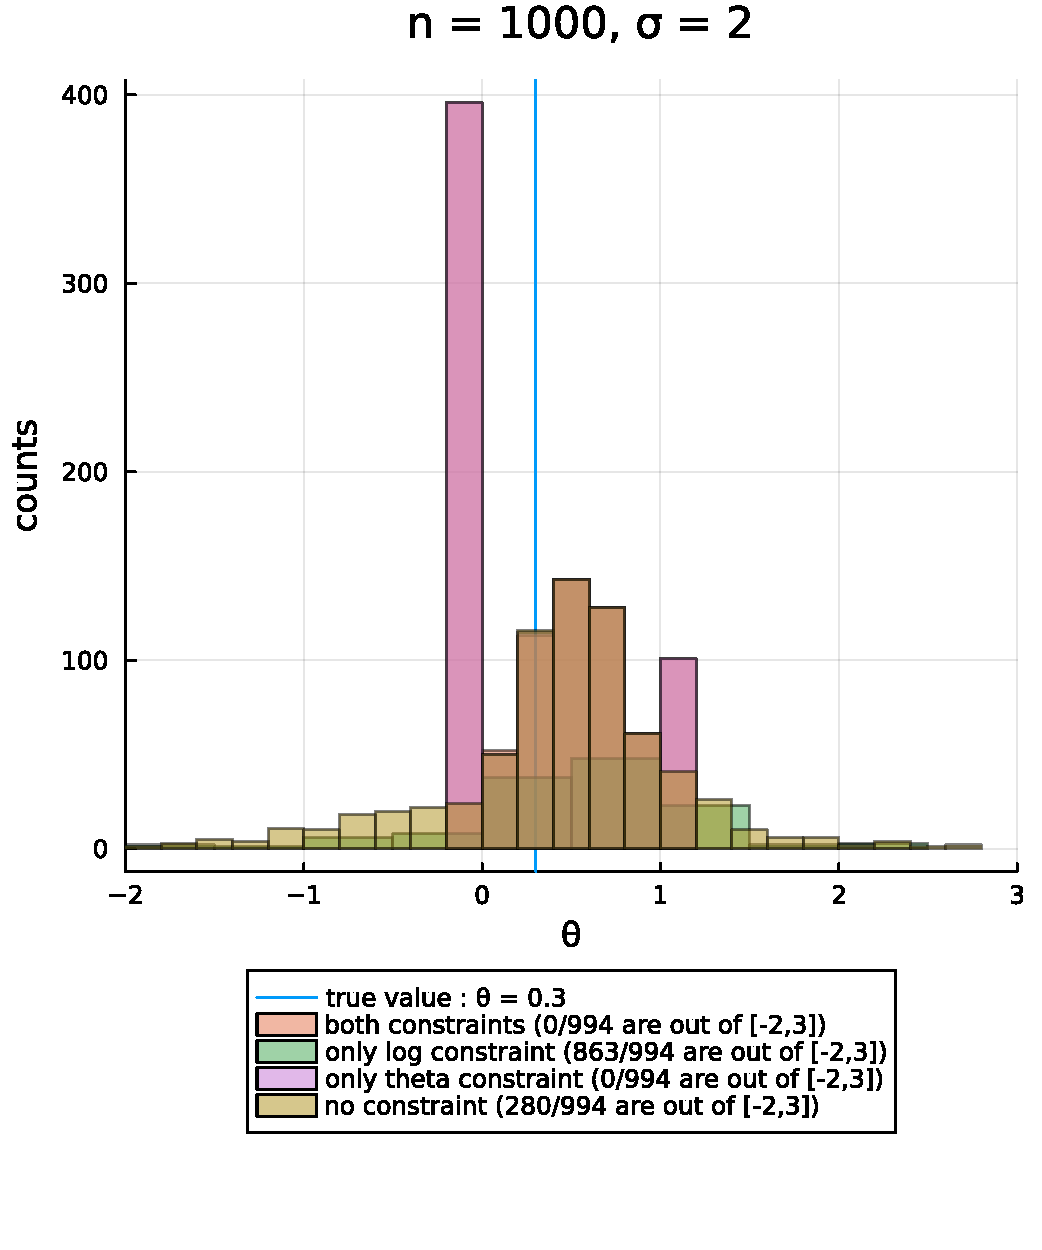
\includegraphics[width = 0.7\textwidth]
  {figuretable/histogram_loglinear_loglinear_n_1000_sigma_2.pdf}}
  \caption{Estimated conduct parameter $\theta$.}
  \label{fg:histogram_loglinear_loglinear_n_1000_sigma_2} 
  \end{center}
  \footnotesize
  Note: True parameters: $\alpha_1 = \alpha_3 = \gamma_0 = \gamma_1 = \gamma_2  = \gamma_3 = 1, \alpha_0 = 10, \alpha_2 = 0.1,  \theta = 0.3.$
\end{figure} 


\begin{figure}[!htbp]
  \begin{center}
  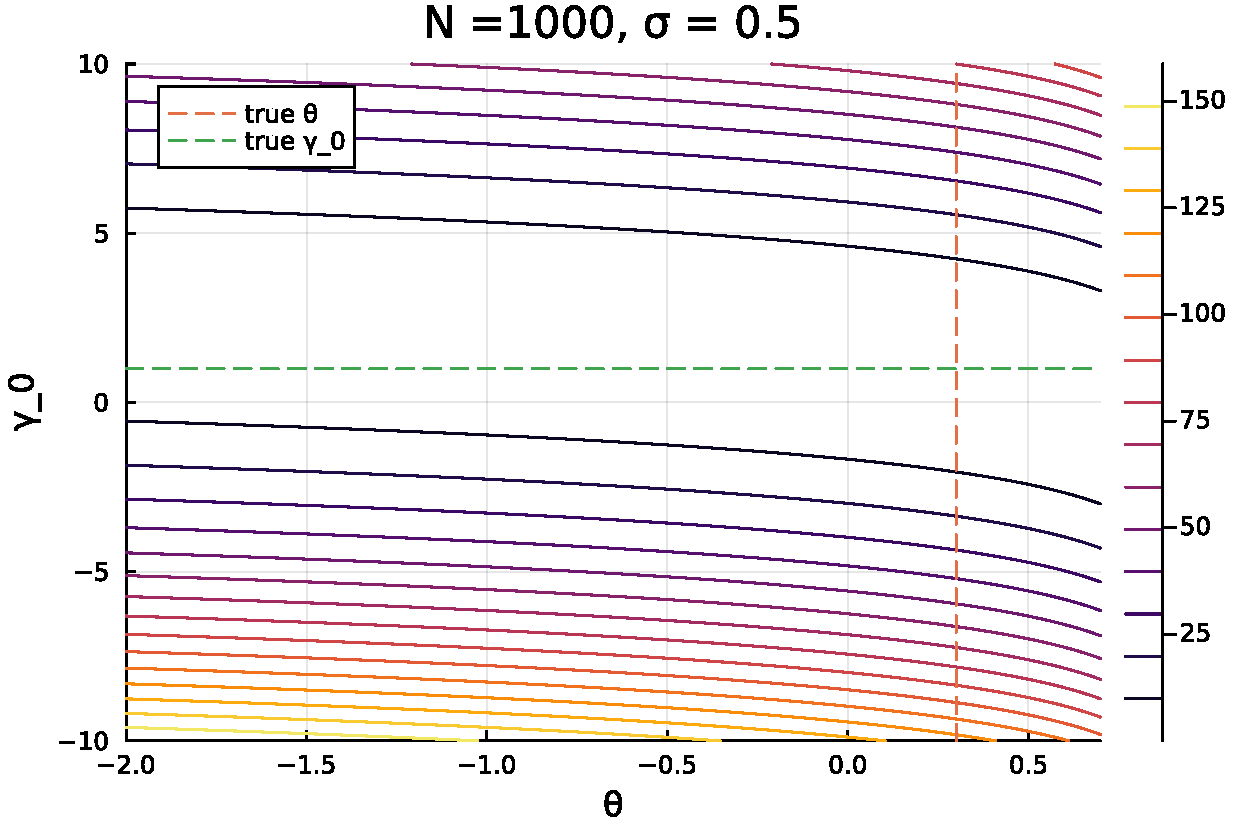
\includegraphics[width = 0.45\textwidth]
  {figuretable/contour_loglinear_loglinear_n_1000_sigma_0.5.pdf}
  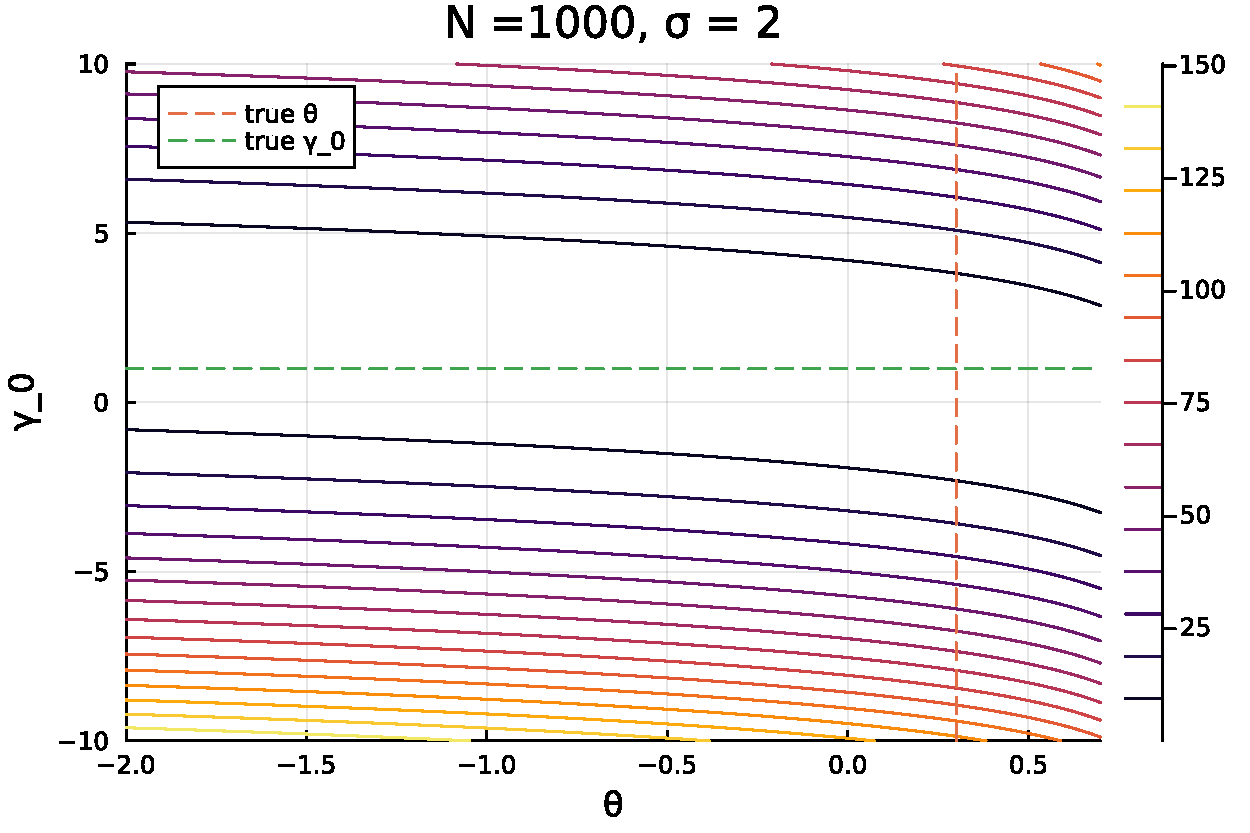
\includegraphics[width = 0.45\textwidth]
  {figuretable/contour_loglinear_loglinear_n_1000_sigma_2.pdf}
  \caption{Contour map of GMM objective function without parameter constraint}
  \label{fg:contour_loglinear_loglinear_n_1000_sigma_2} 
  \end{center}
  \footnotesize
  Note: True parameters: $\alpha_1 = \alpha_3 = \gamma_0 = \gamma_1 = \gamma_2  = \gamma_3 = 1, \alpha_0 = 10, \alpha_2 = 0.1,  \theta = 0.3.$
\end{figure} 



We provide the reason why the estimated conduct parameter has a large standard deviation even if the sample size increases. 
Figure \ref{fg:histogram_loglinear_loglinear_n_1000_sigma_2} illustrates histograms of the conduct parameter from all simulations.
Panel (a) and (b) fix the sample size in each simulation as 1000 but each panel has different values of the standard deviation, $\sigma = 0.5$ and $2$.
Each panel has two histograms of the conduct parameter from the estimation with and without parameter constraint $\theta \in [0,1]$.

As for without constraint, the histogram has a peak abound the true parameter, but we also see samples whose values are less than zero and larger than one.
Note that theoretically, the range of the conduct parameter is between zero and one. 
While the range of the histograms is $\theta \in [-2, 3]$,  we also observe extreme values such as $\hat{\theta} = -10^{15}$ and $10^{8}$.

% About XX% of simulation result is out of the theoretical parameter range [0,1].


Why do such extreme values happen without the parameter constraint?
Figure \ref{fg:contour_loglinear_loglinear_n_1000_sigma_2} illustrates the contour map of the GMM objective function  with respect to $\gamma_0$ and $\theta$.
To draw the map, we fix the other demand and cost parameter values to the true values and set the grid size to 0.01.
we can see that the contour map has a flat region around the true parameters.
Especially, even though we change the value of $\theta$, the GMM value does not change around the true value of $\gamma_0$.

As we mentioned, the value of the estimator of the conduct parameter can take very large or very small values.
Do such values minimize the GMM objective function?
To check this, for each simulation, we the absolute difference between the true parameter values and the value of the estimators and the absolute difference between the value of the GMM objective function under the true parameter values and the estimation result.
Figure \ref{fg:diff_gmm_loglinear_loglinear} shows the plot of these differences. 
Each dot corresponds to each simulation and the color of each dot represents the value of the difference. 
The darker a dot is, the lower the difference is.
We expect that when the difference between the true parameter value and the estimation result is small, the difference of the value of the GMM function is samll, which implies that the color of the dot is darker. 
However, we can see dark dots even when the difference in the conduct parameter is large.
For example, when $\sigma = 0.5$, dark dots appear when the difference is more than 5000.
Furthermore, when $\sigma = 2$, dark dots appear even when the difference is more than 100,000.

While \citet{lau1982identifying} shows the joint identification result of the conduct parameter and the cost parameter in a general case, given Figure \ref{fg:contour_loglinear_loglinear_n_1000_sigma_2} and \ref{fg:diff_gmm_loglinear_loglinear}, we see that the estimation of the conduct parameter and the cost parameter without imposing parameter restriction faces difficulties.





\begin{figure}[!htbp]
  \begin{center}
  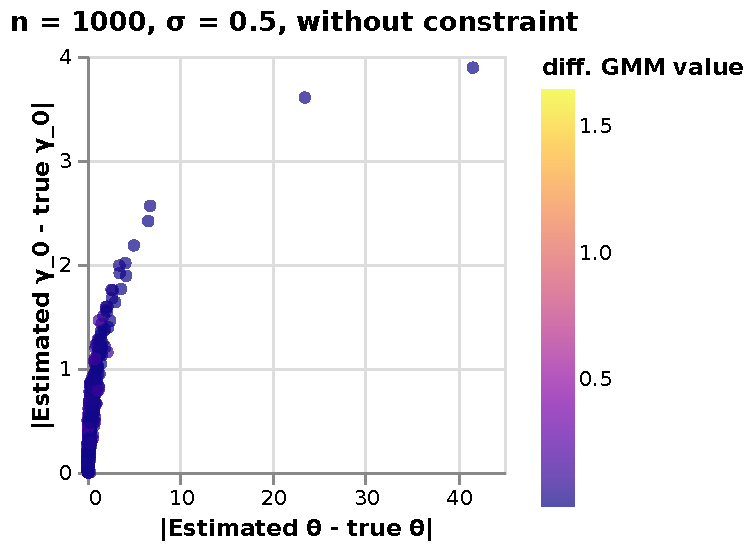
\includegraphics[width = 0.45\textwidth]
  {figuretable/diff_gmm_value_loglinear_loglinear_n_1000_sigma_0.5_non_constraint.pdf}
  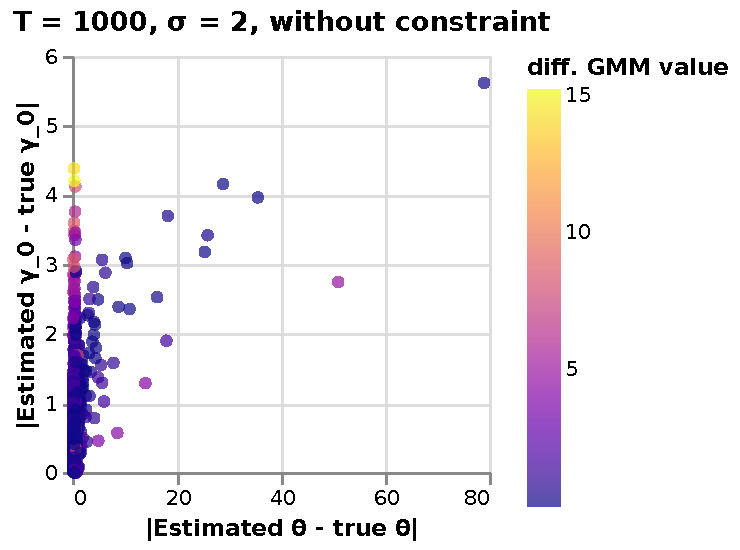
\includegraphics[width = 0.45\textwidth]
  {figuretable/diff_gmm_value_loglinear_loglinear_n_1000_sigma_2_non_constraint.pdf}
  \caption{The difference of the GMM objective function under true parameter and the estimation result}
  \label{fg:diff_gmm_loglinear_loglinear} 
  \end{center}
  \footnotesize
  Note: The x-axis is the difference between the value of conduct parameter estimator and the true conduct parameter. The y-axis is the difference between the value of estimator of $\gamma_0$ and the true parameter. Each dot represents the value of difference of the GMM objective function under the true parameters' values and the values of the estimator. 
\end{figure} 




The above results that $\theta$ estimated by OLS, i.e., without $[0,1]$ domain restriction on $\theta$ can be out of $[0,1]$ are known to the literature. 
For example, \cite{okazaki2022excess} show that estimated $\theta$ is out of $[0,1]$ and the authors explain that conduct parameter estimation is imprecise.





Our paper provides the reason that $\theta$ in log-linear specification is potentially impossible to be jointly identified with cost parameter $\gamma_0$ for the specific data even if we add $[0,1]$ domain restriction. 




Furthermore, detecting collusion or perfect competitive market is imprecise. 
\cite{merel2009measuring} uses log-linear specifications and the estimated $\theta$ is 0.002 with 0.007 standard error, which means perfect competitive markets. 
This may encounter non-identification problem and estimation fails in the boundary as in Figure \ref{fg:histogram_loglinear_loglinear_n_1000_sigma_2}. 
Thus, the suggestion of log-linear specification in \cite{perloff2012collinearity} adds another identification problem. 



Next, Figure %constraint付きのヒストグラム
is the histograms of the conduct parameter from the estimations with parameter constraint, $\theta \in [0,1]$.
For the values in $(0,1)$, the shape of histogram is the same with Figure XXXXXX, but we can see the spike at $\theta = 0$ and $\theta = 1$.
This is simply because the estimation results out of the bound



In summary, we conclude that only the linear model can achieve a proper estimation of the conduct parameter in homogeneous good markets. 




% \paragraph{Yuri Julia}
% \begin{itemize}
%     \item $w \sim U(1,3)$,$r \sim U(0,1)$, and $Z \sim U(0, 1)$. The demand shifter $Y_t$ is drawn from the standard normal distribution
%     \item Two additional random variables are created by adding a random variable drawn from the standard normal distribution to $w$ and $r$
% \end{itemize}



% \paragraph{Suguru R}
% \begin{itemize}
%     \item $w\sim U(1,3) $, $r\sim U(0,1) $, $y\sim N(0,1) $, $z\sim U(0,1) $, $iv_{w}=w+N(0,1) $, $iv_{r}=r+N(0,1) $
%     \item $\theta=0.3$ and $\alpha_2=0.1$ and other parameters are the same as linear case
% \end{itemize}

% \section{MPEC for constrained GMM}

% \begin{itemize}
%     \item separate
%     \item separate, [0,1]constraint
%     \item separate, logconstraint
%     \item separate, [0,1]constraint,logconstraint
% \end{itemize}

    
\section{Conclusion}

We revisit the conduct parameter estimation in homogeneous goods market. In contrast to the pessimistic simulation results shown in \cite{perloff2012collinearity}, our simulation shows that the estimation becomes accurate by properly adding demand shifters in the supply estimation and increasing the sample size. We also show that log linear model recommended by \cite{perloff2012collinearity} has another identification problem. Based on numerical investigation, we conclude that only the linear model can achieve a proper estimation of the conduct parameter in homogeneous good markets. 


\bibliographystyle{aer}
\bibliography{conduct_parameter}


\end{document}